\documentclass[../main/main.tex]{subfiles}


\begin{document}



\section{March 26th, 2019}
\subsection{Flow Decomposition}

\begin{lemma}
	Let $\left( G=(V,E),s,t,c \right) $ be a flow network. Let $f$ be a flow in this network. Then there is a collection of feasible flows  $f_1,f_2,\ldots f_k$ and a collection of $s-t$ paths $p_1,\ldots,p_k$.
\end{lemma}
\begin{itemize}
	\item Value of $f$ is equal to the sum of flows $f_i$.
	\item flow $f_i$ sends positive flow along edge $p_i$.
	\item  $k\le |E|$. (look at lecture notes) for every path, at least one edge will drop off (since once edge gets zero'd, as such we can only have at most $|E|$ paths.
\end{itemize}

This means the average flow \textbf{for the first step} must have $\frac{|f|}{k}$, and the maximum must have more than this amount. This is greater than $\frac{OPT}{|E|}$.

\begin{corollary}
	\label{begMinEdgeCap}
	At the beginning, there is a augmenting path from $s$ to $t$ in which each edge has \textbf{capacity} $\frac{OPT}{|E|}$, where $OPT$ is the value of the maximum flow.
\end{corollary}

This is because there must be a $s-t$ path on the residual network for which all edges on that path has capacity greater than equal to $\frac{OPT}{|E|}$ (as we can push this much flow). 

Since $OPT$ is changing, even though we need at most $|E|$ iterations, running time will be $|E|\log OPT$.

 \begin{theorem}
	 Assuming a flow network with integer capacities, the fattest-path implementation of Ford-Fulkerson method runs in time at most $\left( |E|\log \left( OPT \right) |E|\log |V| \right)=O(|E|^2\log |V| \log (OPT) $ which is polynomial.
\end{theorem}
The time for one iteration to find the largest path is
\begin{itemize}
	\item $|E|$ to construct the residual network
	\item $|E|\log |V|$ to run Dijkstra's algorithm to find the path 
\end{itemize}

\begin{proof}
Let $m=|E|$ and  $f_i$ denote the flow value after $i$ iterations. Let $res_i$ denote the value of optimal flow in the residual network after $i$ iterations.\[
res_i=OPT-f_i
.\] 
By \ref{begMinEdgeCap}, in the ($i$+1)-th iteration, we can find a flow of value greater than or equal to $\frac{res_i}{2|E|}$, as the residual network is a flow network with at most $2|E|$ edges (a forward edge and backward edge for each edge in  $G$). Note that  \[
	res_{i+1}\le res_i-\frac{res_i}{2|E|}=res_i\left( 1-\frac{1}{2|E|} \right) 
.\] As the fattest path has at least $\frac{res_i}{2|E|}$. Now we need to see how many iterations will it take for $res_i$ to be less than or equal to 1 (since they are integer). Note that the factor it drops by is constant. As such we have \[
res_0 = OPT
.\] \[
res_t \le res_{t-1}\left( 1-\frac{1}{2|E|} \right) =\ldots=res_0\left( 1-\frac{1}{2|E|} \right)^{t}=OPT\left( 1-\frac{1}{2|E|}	\right)^{t}.\] 
After $2|E|\ln\left( OPT \right) $ iterations\[
	res_t\approx OPT\left( 1-\frac{1}{2|E|} \right) ^{2|E|\ln OPT}\approx\left( \frac{1}{e} \right) ^{\ln OPT}=1
.\] 
\end{proof}
As such for  $t\approx 2|E|\ln OPT+1$, $res_t<1\implies res_t=0$. Look at formal proof in notes.

The $\log(OPT)$ factor in the running time is awkward for many people, so we will try to remove it.

\subsection{Edmonds-Karp Algorithm}
\begin{definition}[Strongly Polynomial vs Weakly Polynomial]
	An algorithm runs in \textbf{strongly} poly time if, assuming unit time arithmetic operations (e.g. $+,-$), the running time is polynomial in the  $\#$ of numerical operations given as input (polynomial only in $|V|,|E|$).
\end{definition}
Note that our algorithm is not strongly polynomial - we say that it is weakly polynomial. (polynomial in the number of bits in the problem size).\\ 

This distinction is only applicable to problems dealing with integers. One problem where this is relevant is in linear programming. As of now, there are no strongly polynomial time algorithm known yet. All known poly-time algorithms are weakly polynomial (ellipsoid method, integer point methods are weakly polynomial). However, for NP-Complete perspective, both are polynomial in the input size.

Edmonds-Karp Algorithm is a:
\begin{itemize}
	\item Strongly polynomial
	\item Specific implementation of FF method
	\item At each iteration, choose the path in the residual network with the smallest $\#$ of edges. Each iteration will take $|E|$ time (by BFS).
\end{itemize}

\begin{theorem}
	If, at a certain iteration, the length of a shortest $s-t$ path is $\ell$ then at every subsequent iteration, it is $\ge \ell$. Furthermore, after at most $|E|$ iterations, then the length of the shortest $s-t$ path becomes $\ge \ell+1$.
\end{theorem}
	Note that $\ell$ can only stay the same or increase. In addition, at each $\ell$ you can only stay at the same length for $|E|$ iterations. On top of that, $\ell\le |V|-1$, since it is a simple path, as such: \[
		\text{Total }\#\text{ of iterations}\le |E|\left( |V|-1 \right) =O(|E|| V|)
	.\] 
\begin{proof}
	Consider the residual network after $T$ iterations. The length of the shortest $s-t$ path is $\ell$. Edges in the graph of BFS from $s$ that go downwards are called the "forward edges". Note that edges can only go down by one level and can connect vertices on the same level or upwards (cannot go more than one level down).\\
\begin{figure}[h!]
	\centering
	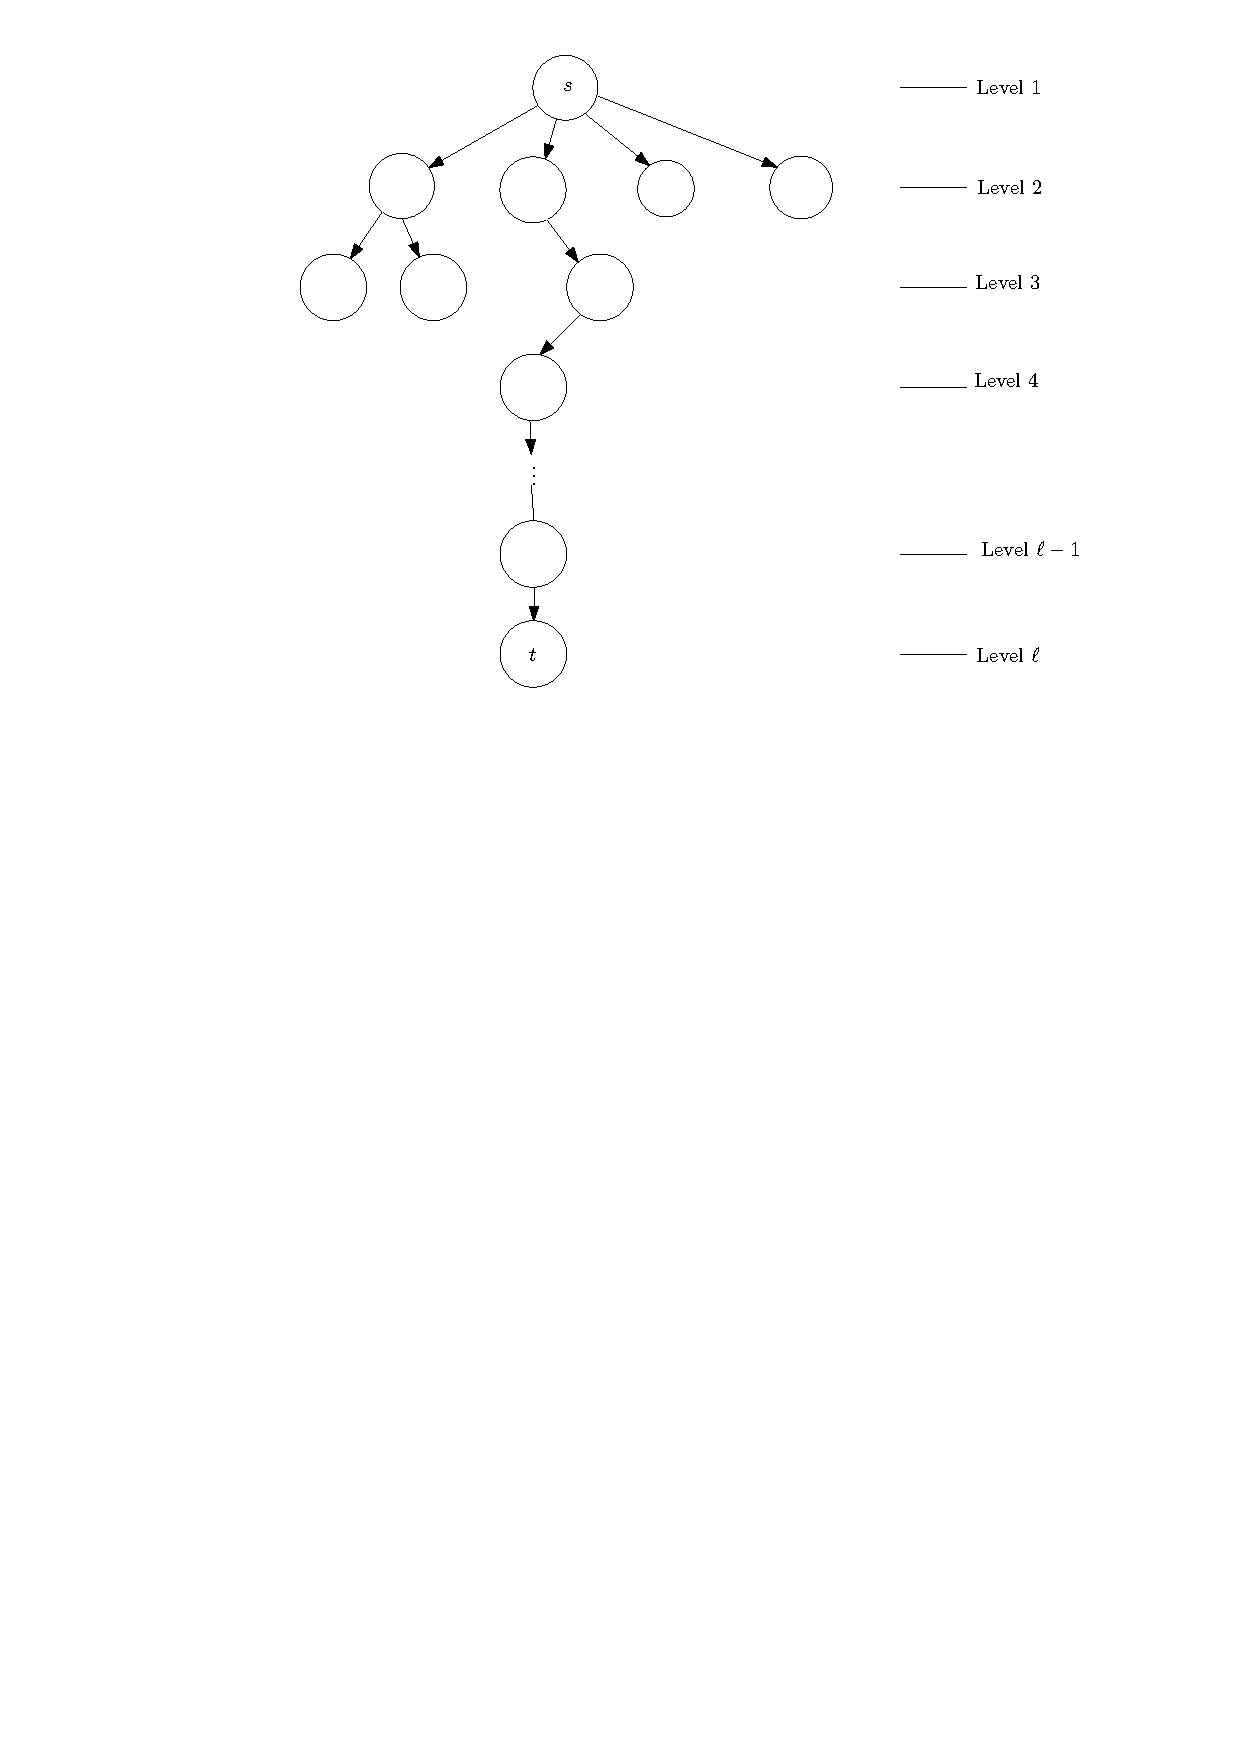
\includegraphics[width=0.5\textwidth]{3-26-BFS.pdf}
	\caption{}
	\label{fig:}
\end{figure}
	In iteration $T+1$, we push additional flow to the shortest $s-t$ path, saturating at least one of the edges on this path. As such the residual network will look as follows:
	\begin{itemize}
		\item All edges on $P$ that are saturated disappear
		\item we may introduce backward edges connecting to edges in $P$
	\end{itemize}
	Note that it will not fall. Proving that $\ell$ is increasing. For $\ell$  to stay the same, you must only use forward edges, otherwise it would increase. Since you remove at least one forward edge during each iteration, you can only stay on the same level for $|E|$ iterations.
\end{proof}
\end{document}
